\section{Introduction}
\label{intro}
The accurate and efficient segmentation of water bodies in very high-resolution satellite and aerial images is critical for various applications in remote sensing, including environmental monitoring, urban planning, and disaster management.\cite{intro1} Remote sensing technologies provide valuable tools for acquiring detailed spatial information over large areas, enabling precise analysis and decision-making. However, the complex nature of high-resolution imagery poses significant challenges for traditional image processing techniques, necessitating the adoption of advanced machine learning models for accurate and automated segmentation tasks.\cite{intro2}\cite{res1}

In recent years, deep learning has emerged as a powerful paradigm in image analysis, offering state-of-the-art solutions for semantic segmentation tasks\cite{res2}. Among the deep learning models, DeepLabv3+ has shown exceptional performance in segmenting objects with fine details and boundaries. This thesis focuses on enhancing the segmentation accuracy of water bodies by leveraging the DeepLabv3+ model and introducing a novel ensemble technique.

The primary objective of this research is to investigate the effectiveness of an ensemble approach using ResNet50V2, MobileNetV3, and EfficientNetV2 as backbones in the DeepLabv3+ architecture. By employing a weighted averaging ensemble method, we aim to capitalize on the unique strengths of each backbone: ResNet50V2 for its robust feature extraction capabilities, MobileNetV3 for its computational efficiency, and EfficientNetV2 for its superior scaling properties. This ensemble strategy is expected to improve the model's ability to capture intricate details and variations in water region imagery, leading to enhanced segmentation accuracy and robustness.
Accurate and timely identification of water bodies is a critical component of management. Traditional methods for water mapping, such as ground surveys and hydrological modeling, are often time-consuming, labor-intensive, and limited in spatial coverage\cite{res3}. Remote sensing technology, which involves acquiring and analyzing satellite or aerial imagery, has emerged as a powerful tool and mapping due to its ability to provide large-scale and real-time data\cite{res4}.
Recent advancements in artificial intelligence \cite{intro3}, particularly deep learning, have further enhanced the potential of remote sensing for water bodies segmentation. Deep learning models, with their ability to automatically learn and extract complex features from raw data, have shown great promise in various image analysis tasks. Among these models, convolutional neural networks (CNNs) have been particularly successful in the field of image segmentation.

This thesis focuses on the application of DeepLabV3+, a state-of-the-art deep learning model, for water bodies segmentation from remote sensing imagery. DeepLabV3+ is a semantic segmentation model that utilizes atrous convolution and spatial pyramid pooling to capture multi-scale contextual information. The model employs ResNet-50 as its encoder for feature extraction, significantly enhancing its ability to produce accurate segmentation maps.\cite{intro4}

The primary objective of this research is to develop and evaluate a robust segmentation model that can accurately delineate water affected areas from satellite images. A comprehensive dataset comprising multi-spectral satellite images and corresponding ground truth annotations was used to train and validate the model. The performance of DeepLabV3+ was assessed using metrics such as Intersection over Union (IoU), precision, recall, and F1 score.

The results of this study demonstrate that DeepLabV3+ achieves high accuracy in water bodies segmentation, outperforming traditional image processing techniques and other segmentation models. By leveraging advanced deep learning methodologies, this research contributes to the development of more effective flood response strategies and disaster management practices. Future work may involve integrating additional data sources, such as topographic and meteorological data, to further enhance model accuracy and predictive capabilities.

\section{Framework/Design Overview}
The proposed methodology for water bodies segmentation using DeepLabV3+ is a comprehensive approach designed to accurately identify and delineate water areas within satellite or aerial images. It begins with the collection and preparation of the dataset, which involves gathering images along with corresponding ground truth masks, resizing the images, and encoding the masks for training purposes. The model selection phase focuses on choosing DeepLabV3+ as the semantic segmentation model, utilizing pre-trained ResNet50V2, EfficientNetV2, MobileNetV3 backbone to leverage transfer learning. The overview of all methodology steps is presented in this section and \ref{metho1} represents the block diagram of the proposed model.
\\

\begin{figure}[H]
\centering
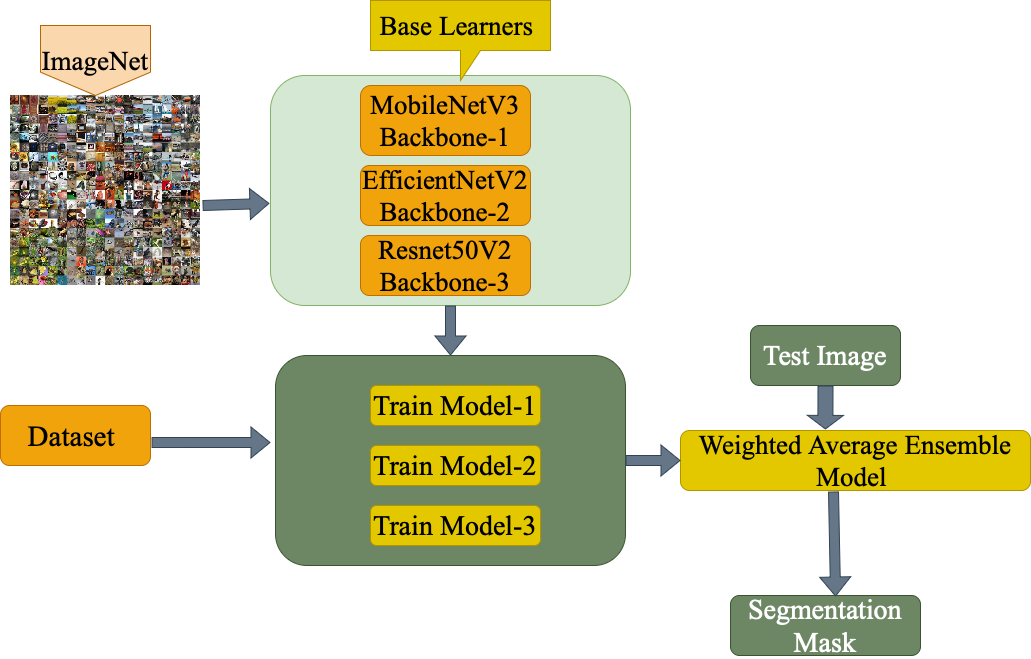
\includegraphics[width= 1\textwidth]{figs/first-3.png}
\caption{Proposed Framework}
\label{metho1}
\end{figure}




\section{Difficulties}
There are always some difficulties while working with deep learning methods and different dataset.Our thesis project on water bodies segmentation is crucial as it provides a realistic account of the challenges faced and how they were addressed.
A list of some of the most common challenges is provided below:
\begin{enumerate}
       \item \textbf{Data Collection :} Finding sufficient and high-quality satellite images, drone footage and normal images as well as their corresponding masks were challenging.
        \item \textbf{Data Quality :} Differences in image resolution affected the consistency and accuracy of the segmentation results.
        \item \textbf{Annotation and Labeling :} Ensuring consistent and accurate labeling across the dataset were difficult, especially with complex scenes.
        \item \textbf{Finding the appropriate model :} Numerous candidate models with different parameters that can be adjusted in different ways to improve performance are available. Therefore, a large number of experiments must be conducted in order to identify the effective model.
        \item \textbf{Model Development :} Fine-tuning hyperparameters for the optimal model performance was computationally intensive and required significant resources.
        \item \textbf{Overfitting :} It's crucial to stop overfitting when the DNN model is being trained. It is necessary to use methods like cross-validation and regularization to make sure the model performs effectively when applied to new data.
        \item \textbf{Training the model :} It requires a significant amount of time and machine configurations to train many models with varying parameters. Finding the ideal parameters and model for our architecture grew more difficult as a result.

\end{enumerate}


\section{Applications}


\begin{itemize}
    \item \textbf{Environmental Monitoring:} Accurate segmentation of water bodies can aid in monitoring water quality parameters such as turbidity, sedimentation, and pollution levels. This information is crucial for assessing environmental health and implementing remedial measures.
    Identifying and mapping water bodies helps in understanding aquatic habitats and ecosystems, supporting biodiversity conservation efforts.
    \item \textbf{Urban Planning and Infrastructure Management: } Precise delineation of water bodies assists in managing water resources, including allocation for drinking water supply, irrigation, and industrial use.
    \item \textbf{Flood Risk Assessment: } Mapping water bodies contributes to flood risk assessment and mitigation strategies, allowing urban planners to better plan infrastructure and develop early warning systems.
    \item \textbf{Disaster Management:} During natural disasters such as floods or hurricanes, accurate maps of water bodies facilitate emergency response operations, evacuation planning, and assessing the extent of damage.
     After disasters, monitoring changes in water bodies helps in assessing environmental impact, planning restoration efforts, and prioritizing resource allocation.
     \item \textbf{Agriculture and Land Use Planning:} Identifying water bodies aids in planning irrigation systems and optimizing agricultural practices, ensuring efficient water use in agriculture.
     \item \textbf{Infrastructure Development and Engineering:} Accurate mapping of water bodies informs decisions on infrastructure development projects such as dams, bridges, and roads, minimizing environmental impact and optimizing construction planning.
     \item \textbf{Hydrological Modeling: }Detailed water body segmentation supports hydrological modeling for flood forecasting, groundwater recharge estimation, and watershed management.
     \item \textbf{Remote Sensing and GIS Applications: }Water body segmentation is essential for creating detailed and up-to-date maps used in GIS applications for various purposes, including navigation, tourism, and land use planning.
    
\end{itemize}

\section{Objectives}
The objectives are designed to address key challenges in water bodies segmentation and to develop a practical, accurate, and user-friendly model that can be utilized in various real-world applications.The key objective and possible outcomes of this work are mentioned below:
\begin{itemize}
    \item To design and implement a robust model for accurately segmenting water areas in satellite or aerial imagery.
    \item To improve existing image processing techniques or develop new ones for better feature extraction and classification of water regions.
    \item  To rigorously evaluate the performance of the segmentation model using various metrics, such as accuracy, precision, recall, and F1 score, Mean IoU.
    \item  To test the segmentation model in real-world scenarios and assess its applicability for various use cases.
    \item  To identify and analyze the challenges and limitations encountered during the development and implementation of the segmentation model.
\end{itemize}

\section{Motivation}
Accurate segmentation of water bodies supports various environmental monitoring applications, including assessing water quality, monitoring changes in aquatic habitats, and understanding the impacts of climate change on hydrological systems. These applications are crucial for informed decision-making in environmental management and policy.With the increasing availability and volume of satellite imagery, there is a growing demand for automated and efficient methods to analyze and interpret these vast datasets. Automated segmentation of water bodies reduces manual effort, accelerates analysis processes, and improves the consistency and accuracy of results.

The factors that led us to motivate for this work :

\begin{itemize}
        \item One of our main motivations was traditional water monitoring methods can be slow and resource-intensive. There is a growing need for advanced, automated tools that can quickly and accurately identify water region areas, helping authorities to respond more effectively to these events.
        \item Water bodies, such as lakes, rivers, and reservoirs, are crucial natural resources that support various ecosystems and human activities. Accurate mapping and monitoring of these water bodies are essential for effective water resource management, environmental conservation, and disaster preparedness.
        \item Advances in remote sensing technology and machine learning have created new opportunities for developing sophisticated water detection systems. Leveraging these technologies can enhance our ability to monitor and manage flood risks.
        \item Climate change is contributing to more frequent and severe flooding events. Developing robust water segmentation models is essential for preparing and adapting to these changing environmental conditions.
        \item Despite the advancements in deep learning for image segmentation, there may still be gaps in achieving optimal accuracy and efficiency, especially in the context of diverse and challenging environmental conditions. Your thesis aims to fill this gap by proposing and evaluating an innovative ensemble approach to enhance water body segmentation performance.
        

       
\end{itemize}
\section{Contribution of the thesis}
The contributions of this thesis are multifaceted, addressing both theoretical and practical aspects of water bodies segmentation. By developing a robust and accurate segmentation model, integrating multi-source data, and providing an end-to-end solution for real-time water monitoring, this research makes significant advancements in the field. The primary contribution of this thesis is the following:
\begin{enumerate}
    \item \textbf{Development of a Robust Segmentation Model : }This thesis develops a novel segmentation model using deep learning techniques. The model is capable of accurately identifying and delineating water areas from satellite or aerial imagery, offering improvements over existing methods in terms of accuracy and computational efficiency.
    \item \textbf{Integration of Multi-Source Data : }The research integrates data from various sources, such as satellite imagery, weather data, and topographical information, to enhance the model's performance. This multi-source data fusion helps in achieving more reliable and comprehensive water mapping.

    \item \textbf{Application of Advanced Machine Learning Techniques : }The architecture of the neural networks was fine-tuned by experimenting with different numbers of layers, filter sizes, and activation functions to find the optimal configuration for the segmentation.
\end{enumerate}

\section{Thesis Organization}
The complete report is divided into five chapters. The report structure may be summarized as follows:
\begin{itemize}
    \item \textbf{Chapter 1} provides a general description of research and discusses the obstacles, motivation, and application of the work.
    \item \textbf{Chapter 2} outlines and compares the technology employed in our works with some related works
    \item \textbf{Chapter 3} describes the technique and illustrates the system’s implementation
    \item \textbf{Chapter 4} discusses the experimental results and analysis of the experiment.
    \item \textbf{Chapter 5} contains the conclusion of this work which includes an overall overview of our system and also mentions some limitations \& future work.
\end{itemize}






\section{Conclusion}
We provided a thorough description of the design in this chapter, covering its conception, problems that were found, possible uses, and contributions to the world at large. We also discussed the work's larger context and significance, highlighting its relevance, goals, and possible ramifications.
